\documentclass{article}

% Times font, math in Times Italic
% TODO: Not actually very happy with some of the typesetting, especially around sums in equations
\usepackage{mathptmx}
\usepackage{mathtools}
\usepackage{amsfonts}
% Generate PDF links for ToC, cite, ref, etc.
\usepackage{hyperref}

% This somehow takes advantage of pdftex features and magically make the document typeset nicer,
% for example it's managed to resolve an underfull hbox warning on its own.
\usepackage{microtype}

% To get nice numbered algorithm floats
\usepackage{algorithm}
% To actually typeset algorithms
\usepackage{algpseudocode}

% Theorem styles
\usepackage{amsthm}

\usepackage{graphicx}
\usepackage[outdir=./out/]{epstopdf}
\graphicspath{ {./images/} }
\usepackage{subcaption}

% Prevent single first or last lines of a paragraph appearing alone at the top or bottom
% of a page.
\clubpenalty=10000
\widowpenalty=10000

% We get a bunch of underfull hboxes is the references, which seem hard to impossible to fix nicely,
% so this silences them for now so they're not spamming the output.
% TODO: Before actual submission, turn this off and try and fix any underfull hbox reported. If some
% can't be fixed, that's not big deal either.
\hbadness 10000

% This declares \abs and \norm commands
\DeclarePairedDelimiter\abs{\lvert}{\rvert}%
\DeclarePairedDelimiter\norm{\lVert}{\rVert}%

% Swap the definition of \abs* and \norm*, so that \abs
% and \norm resizes the size of the brackets, and the 
% starred version does not.
\makeatletter
\let\oldabs\abs
\def\abs{\@ifstar{\oldabs}{\oldabs*}}
%
\let\oldnorm\norm
\def\norm{\@ifstar{\oldnorm}{\oldnorm*}}
\makeatother

\newcommand{\todo}[1]{\paragraph{TODO} #1}

% Number definitions, theorems, and lemmas with a single counter.
\newtheorem{theorem}{Theorem}[section]
\newtheorem{lemma}[theorem]{Lemma}
\theoremstyle{definition}
\newtheorem{definition}[theorem]{Definition}

\title{Thesis}
\author{Sebastian Paarmann}
\date\today

\begin{document}

\maketitle

\tableofcontents

\todo Typesetting of "Infinity"

\section{Introduction}

A \emph{cluster} graph, also called \emph{transitive} graph, is a graph which consists only of
disjoint cliques.  In the \textsc{Cluster Editing} problem, the input is an undirected graph $G$ and
an integer $k \geq 0$, and the question is whether the $G$ can be made into a cluster graph using
$k$ or less \emph{edge edits}. An edit is either inserting an edge or deleting an existing one. We
also consider the \textsc{Weighted Cluster Editing} problem: The input has weights for each edge and
non-edge, which are the deletion and insertion costs respectively. The question is then whether
there is a solution with total edit costs at most $k$.

\todo Problem of finding the optimal solution without having a $k$ given

\todo This introduction needs some more work, could be a bit more clear and probably want a
formal formulation of the problem somewhere (symmetric difference of edge sets etc.)

\todo Motivation for the problem, practical applications

\todo Should mention the PACE challenge somewhere here

First, some notation used throughout: A graph $G = (V, E)$ has a vertex set $V$ and edge set $E
\subseteq \binom{V}{2}$. Graphs are simple graphs, i.e.\ they contain no self-loops or parallel
edges.  We abbreviate an edge or non-edge $\{u, v\} \in \binom{V}{2}$ as $uv$. We denote the (open)
neighborhood of a vertex $v$ in $G$ as $N_G(v)$. Similarly, $N_G[v]$ is the closed neighborhood
of~$v$, i.e.\ $N_G(v) \cup \{v\}$. If it is clear which graph is meant, we may also just write
$N(v)$ and $N[v]$.  A weighted graph $G$ is characterized by a weight function $s\colon \binom{V}{2}
\to \mathbb{Z}$. We consider $uv$ to be an edge if $s(uv) > 0$ and $uv$ to be a non-edge if $s(uv)
\leq 0$.

\todo Notation paragraph needs some cleanup; and at the end make sure this has everything relevant
that's used and nothing that isn't.
\todo More notation: Induced graphs, symmetric differences, $N^2(v)$

\textsc{Cluster Editing} is NP-complete
\todo Cite, APX-hardness, existing approximations(?)

\todo fpt approaches and fpt-tractability, including how you keep increasing k etc.
\todo What a kernel is

A very simple FPT algorithm is given by the observation that a graph $G = (V, E)$ is a cluster graph
if and only if there is no \emph{conflict triple} in the graph. Three vertices $v, u, w \in V$ form
a conflict triple if $uv, uw \in E, vw \notin E$. The problem can be solved by recursively searching
for a conflict triple and branching into three cases: Add $vw$, remove $uv$, or remove $uw$. These
are the only ways of resolving a conflict, and once there are no more conflicts, a solution can be
returned. With an upper bound $k$ for the number of edits as described above, this gives a search
tree of size $3^k$.

\todo Should this be here? Should it be somewhere else?

\todo Image for a conflict, and its resolutions, maybe (in general some visualizations would be
nice)

%todo Should decide on consistent rules for using $O(k)$ vs $O(k + n + m)$ etc., and apply these to
%existing text.

\section{Previous Work}

\todo There are still a few things missing from this: \begin{enumerate}
	\item ILP formulations
	\item The $1.92^k$ algorithm
	\item Work after the golden ratio paper, including e.g.\ the paper by Hartung and Hoos, among
		others.
\end{enumerate}

%todo Maybe change listing of 3 authors to et al.?

Clustering problems in general have a very long history, so we will focus only on the specific
\textsc{Cluster Editing} problem as formulated above. In 1999, Ben-Dor, Shamir, and
Yakhini~\cite{BenDor} introduced the unweighted problem in order to perform clustering on gene
expression patterns. They provided a stochastic model for the corruption of the true clustering
introduced by measurements and present an $O(n^2 \log(n)^c)$ algorithm that reconstructs the true
clustering with high probability, as well as a heuristic approach based on a similar idea. Many
other approaches for clustering gene expression data had been proposed and investigated already at
this time, see \cite{ShamirOverview} for an overview from 2001.

Shamir, Sharan, and Tsur~\cite{ShamirModifications} investigated \textsc{Cluster Editing} as well as
the related \textsc{Cluster Completion} (only edge insertions allowed) and \textsc{Cluster Deletion}
(only edge deletions allowed) problems further. They showed that \textsc{Cluster Completion} can be
solved in polynomial time, \textsc{Cluster Deletion} is NP-hard to approximate to within some
constant factor, and, most relevant for us, \textsc{Cluster Editing} is NP-complete.  Additionally
they also considered variants of the problems with a fixed number of clusters as input, which we
will not further consider. Gramm et al.~\cite{Gramm} also mention that the NP-completeness of
\textsc{Cluster Editing} can already be derived from the work of Křivánek and
Morávek~\cite{Krivanek}, published in 1986.

Bansal, Blum, and Chawla independently researched a group of problems they call \textsc{Correlation
Clustering}~\cite{Bansal}. In their formulation, "minimizing disagreements" between the input
labelling and the output clustering is equivalent to the unweighted \textsc{Cluster Editing}
problem, which they give a constant-factor approximation for. This result was improved on in 2005 by
Charikar, Guruswami, and Wirth~\cite{Charikar}, who show the problem to be APX-hard and give an
approximation with a constant factor of 4.

In 2003 Gramm et al.~\cite{Gramm} gave initial results regarding fixed-parameter approaches for
\textsc{Cluster Editing} specifically. Before that, Cai~\cite{Cai} investigated fixed-parameter
tractability of graph modification problems characterized by forbidden subgraphs in a more general
sense, the results of which imply an $O(k^3 * \abs{G}^4)$ algorithm for \textsc{Cluster Editing}.
Gramm et al.\ gave an $O(k^3)$ kernel for the problem, as well as a straightforward $O(k^3 + n^3)$
fixed-parameter algorithm. Additionally they show a more advanced branching strategy that improves
the search tree size to $O(2.27^k)$, leading to an $O(2.27^k + n^3)$ algorithm.  This approach was
implemented in practice for the first time and empirically compared to an LP-based solver by Dehne
et al.\ in 2006~\cite{Dehne}. They find that the $O(2.27^k)$ is indeed faster in practice than the
simpler $O(k^3)$ branching.

Another avenue of research was started in 2007 by Rahmann et al.~\cite{Rahmann}. This introduced the
first fixed-parameter algorithm for the weighted version of the problem, along with several data
reduction rules to speed it up. They also introduced two heuristic algorithms.

Building on this, Böcker et al.\ published several papers in 2008. They introduce a variant of the
refined branching strategy of Gramm et al.~\cite{Gramm} for the weighted problem, resulting in an
$O(2.42^k)$ algorithm~\cite{AnApproach}. Most importantly, this is the first paper to introduce
merging two vertices, which is an operation only possible on the weighted problem. As a result, with
merging, Böcker et al.\ find the simpler $O(3^k)$ branching faster in practice than the refined
branching strategy, largely due to the significant effect of merging. Merging is also the basis for
a very simple $O(2^k)$ branching algorithm~\cite{GoingWeighted} which means the fastest practical
approach to solving the unweighted problem is now to transform it into a weighted instance and solve
that.  The paper also immediately improves upon this with an $O(1.82^k)$ algorithm that is achieved
by more carefully choosing which edge to branch on. This beats even the previous best theoretical
runtime for the unweighted problem of $O(1.92^k)$. Lastly, Böcker et al.\ perform practical
experiments with these algorithms~\cite{ExactAlgos}, comparing them with a cut-and-branch based ILP
implementation.  They find both approaches to be competitive, with different performance
characteristics. Notably, good data reduction rules make the FPT approach feasible even for graphs
that require several thousand edge modifications, despite the worst-case running times.

This basic approach was improved further by Böcker and Damaschke. First, a theorem introduced by
Damaschke~\cite{BoundedDegree} concerning the structure of graphs in which no edge is part of three
conflict triples, is used to improve the algorithm to $O(1.76^k)$~\cite{EvenFaster}. Then zero-edges
(which will be discussed in more detail later) can be used to show additional structural properties,
allowing even more efficient branching for an $O(1.62^k)$ search tree~\cite{GoldenRatio}.

In parallel multiple problem kernels for \textsc{Cluster Editing} have also been developed. Note
that we discuss them here separately only to make it easier to follow, in practice the work on
kernels is often what makes the better algorithms possible: Better reduction rules introduced as
part of a kernel allow constructing and proving a faster search tree algorithm. In fact, these are
often developed as a single work. Such it is for the first kernel given by Gramm et al.~\cite{Gramm},
which has at most $2k^2 + k$ vertices and can be computed in $O(n^3)$ time.

Protti, da Silva, and Szwarcfiter~\cite{Protti} gave a kernel with at most $2k^2 + 4k$
vertices, slightly worse than that off Gramm et al.\ but still $O(k^2)$. It is based on the modular
decomposition of a graph and has the advantage of only requiring running time $O(n + m)$. In 2007,
Fellows et al.\ introduced a "crown-type structural reduction rule"~\cite{Fellows} and show it
can be used to construct a kernel with $6k$ vertices that can be computed in polynomial time.

Based on both the ideas of the crown-type reduction and the concept of \emph{critical cliques},
which had already been used for good effect in fixed-parameter approaches to other problems,
Guo~\cite{Guo} presented first another $6k$ kernel with $O(n^3)$ runtime and immediately improved
this to a kernel with at most $4k$ vertices computable in $O(nm^2)$ time.

Lastly, in 2011, Chen and Meng~\cite{ChenMeng} combined the critical cliques concept with the notion
of an \emph{editing degree} of a vertex to give a $2k$ kernel which runs in $O(nm)$ time.

\section{Our Implementation}

\todo This is missing some attributions right now, most notably for the whole merging thing, but
probably to some extent for other things too.

\todo Should motivate merging more somewhere, setting to "forbidden" and "permanent" being the
intuitive thing and merging just being a cooler version of the latter.

\todo Revisit branching strategy to potentially be based on lowest-branching-number instead

In this section we will describe the implementation of our solver in some detail. It is based on
many techniques introduced by the papers mentioned above. Those are only briefly summarized there
but we will give more detailed information about those we have implemented here.

There are 4 parts of this section: We start off by describing the high-level structure of the
solver, followed by a more in-depth look at the two basic modifying operations that are performed on
the graph during execution of the algorithm. Next, we describe the reduction rules used, and finally
some details on the practical implementation of the described algorithm, e.g.\ used data structures.

\subsection{High-Level Overview}

The solver consists of two main parts: The solver function, Algorithm~\ref{alg:solver}, that
performs interleaved reduction and the branching strategy, calling itself recursively; and a
\emph{driver}, Algorithm~\ref{alg:driver} that splits the input graph into its connected components,
performs some initial reduction and conversion to a weighted instance, and then calls the recursive
solver function with increasing parameter $k$ until a solution is found. 

The reductions are split into several categories. There is the initial step of taking an
unweighted instance and turning it into a reduced weighted instance. A set of parameter-independent
reduction rules can also be applied directly after this, before the main search-tree algorithm.
These parameter-independent rules are also applied interleaved during the search. And finally, any
reductions that depend on having a maximum cost parameter $k$ can be applied only once the search
has started.

During the recursive search, we must track the current graph, which is modified for each recursive
step, the current value for $k$ as well as the set of edits done so far in the current branch.
Because we modify the graph not just by inserting and deleting edges in the course of the algorithm,
but also by merging vertices (which effectively removes a vertex; see below for details), we also
need to keep track of which vertices in the current graph correspond to which vertices of the
original graph. One can either keep tracking edits throughout the branching search in terms of the
original graph, or reconstruct the edit set at the end based on the final graph and the information
about how vertices correspond. Theoretically the latter is more optimal in terms of runtime because
it only needs to do some work once the solution has been found, while the former approach has a
slight overhead while searching. Our testing has indicated the difference is negligible however and
we currently implement the former approach.

\todo Possibly include the test results?

\todo These algorithms kind of swing between by-ref and by-value arguments as they want to, should
formulate this a bit more nicely

\begin{algorithm}{Driver}
\caption{Driver}
\label{alg:driver}
\begin{algorithmic}

\Function{ComputeOptimalClusterEditing}{$G: Graph$}
	\State $edits \gets \emptyset$
	\ForAll{$comp \in \Call{Components}{G}$}
		\State $instance \gets \Call{MakeWeightedInstance}{comp}$
		\State $lb1 \gets \Call{InitialReduction}{instance}$
		\State $lb2 \gets \Call{LowerBound}{instance}$
		\State $k \gets \Call{Max}{lb1, lb2}$
		\Repeat
			\State $solution = \Call{SolveClusterEditing}{instance, k, \emptyset}$
			\State $k \gets k + 1$
		\Until{$solution \neq \emptyset$}

		\State $edits \gets edits \cup solution$
	\EndFor
	\State \Return $edits$
\EndFunction

\end{algorithmic}
\end{algorithm}

\begin{algorithm}
\caption{Recursive Solver}
\label{alg:solver}
\begin{algorithmic}

\Function{SolveClusterEditing}{$instance, k, edits$}
	\If{$k < 0 \lor k < \Call{LowerBound}{instance}$}
		\State \Return $\emptyset$
	\EndIf

	\State $\Call{Reduction}{instance, k}$

	\If{$k < 0 \lor k < \Call{LowerBound}{instance}$}
		\State \Return $\emptyset$
	\EndIf

	\If{$\neg \Call{HasConflictTriple}{instance}$}
		\State \Return $edits$
	\EndIf

	\State $(v, u, w) \gets \Call{GetConflictTriple}{instance}$
	\\
	\State $delInstance \gets \Call{Clone}{instance}$
	\State $delK \gets k$
	\State $delEdits \gets \Call{ForbidEdge}{delInstance, delK, uv, edits}$
	\State $delSolution \gets \Call{SolveClusterEditing}{delInstance, delK, delEdits}$

	\If{$delSolution \neq \emptyset$}
		\State \Return $delSolution$
	\EndIf
	\\
	\State $mergeEdits \gets \Call{MergeEdge}{instance, k, uv, edits}$
	\State $mergeSolution \gets \Call{SolveClusterEditing}{instance, k, mergeEdits}$
	\State \Return $mergeSolution$
\EndFunction

\end{algorithmic}
\end{algorithm}

\subsection{Basic Operations}

Both the reduction rules and the branching algorithm itself only need to perform two kinds of
modifications on the graph: Setting an edge to forbidden, which includes deleting the edge if it
currently exists in the graph; and merging two vertices, which implies setting the edge between them
to permanent but also reduces the size of the remaining graph in the process and can result in
multiple other edits in addition to inserting the edge between the vertices.

% TODO: Might be good to explain the part of tracking edges in terms of original vertices, so that
% even a Delete(u, v) edit can actually produce multiple edits a bit more. Only want to do that once
% Experiment1 is finished and confirms we do keep doing it like that :)

\paragraph{Forbidding} Of the two, forbidding an edge is the much simpler operation. If $uv$
currently exists, deleting it will generate cost. We thus reduce $k$ by $\max\{s(uv), 0\}$. If $s(uv)
> 0$, we record the edit(s) from removing the edge. We then set $s(uv) = -Infinity$ to mark it as
forbidden and prevent it from being reintroduced later.

\paragraph{Merging} \label{sec:merging} Merging two vertices $u$ and $v$ is more complicated. Conceptually, we introduce
a new vertex $u'$ and insert it into the graph while removing $u$ and $v$. Merged vertices are
considered to have a permanent edge between them (we can't later split them apart again), so if
$s(uv) \leq 0$, we record the edit(s) from inserting the edge. This also generates cost, so reduce
$k$ by $\max\{-s(uv), 0\}$. Then, for all $w \in V \setminus \{u, v\}$, we set $s(u'w) = s(uw) +
s(vw)$.

It is possible that before the merge $uw$ existed and $vw$ did not, or vice-versa. In that case,
this merge procedure will also effectively insert or delete one of these edges, depending on their
weights. Any edits resulting from such a case are also recorded as edit, and reduce $k$
appropriately. Note however that while \emph{primary} edits (forbidding or merging $uv$) result in
$uv$s new status being permanent and never changing again (in this part of the search tree), this
kind of \emph{secondary} edit occurring as a side-effect of merging can be changed again later in
the algorithm, by editing $u'w$.

An additional complication is the fact that the described merging procedure can create edges with
weight 0, if $s(uw) = -s(vw)$.
\todo Finish discussing zero-edges

\subsection{Reduction Rules}

\paragraph{Critical Cliques} One can obtain an equivalent weighted instance from an unweighted one,
by simply setting $s(uv) = 1$ for all $uv \in E$ and $s(uv) = -1$ for all $uv \notin E$. We use a
slightly more complex procedure that can already reduce the graph while making it weighted, based on
the notion of \emph{critical cliques}.

\begin{definition}
	A \emph{critical clique} $K$ is an induced clique in $G$ where all vertices of $K$ have the same
	set of neighbors, and $K$ is maximal under this property. 
\end{definition}

An optimal cluster editing never splits a critical clique, i.e. every critical clique $K$ of the
input graph will be contained in a single cluster for any optimal solution~\cite{Guo}. Guo uses this
observation and more to construct a $4k$ kernel for the unweighted cluster editing problem. We can
take advantage of the technique of merging vertices instead: Since all vertices in a critical clique
end up in the same cluster, we can merge every critical clique into a single vertex, which will
transform the unweighted input into an integer-weighted graph. The resulting graph has at most
$4k_{opt}$ vertices, providing a simple lower bound for the parameter at the start of the
algorithm~\cite{GoingWeighted, Guo}.

Finding the critical cliques is possible in $O(n + m)$ time. In practice we implemented a simpler
$O(n^2)$ algorithm: Until all vertices have been assigned to a critical clique, choose one
unassigned vertex to put in a new critical clique, and add every other unassigned vertex with the
same closed neighborhood to the same critical clique. Our implementation time was constrained and
this reduction is only ever executed once for every connected component of the input graph, so we
focused our efforts on parts that have a more significant effect on total runtime instead of
implementing the more complicated $O(n + m)$ algorithm.

\todo Effectiveness of critical clique reduction (this is very easy to measure)

\paragraph{Parameter-independent reduction} As described above, parameter-independent reduction can
be applied once as reduction at the very start of the algorithm, but also during the search tree
algorithm: After some branches in the search tree have been taken, more reduction operations may
become applicable in the context of the current branch. Concretely, we implemented reduction
rules~1--5 as introduced by Böcker et al.~\cite{ExactAlgos}. We repeat the rules here along with
notes about their implementation, but omit full proofs of correctness and runtime.

\todo images 

\subparagraph{Rule 1} \emph{(heavy non-edge rule)} A non-edge $uv$ with $s(uv) < 0$ can be forbidden
if
\[
	\abs{s(uv)} \geq \sum_{w \in N(u)} s(uw).
\]

Intuitively, if adding $uv$ is more expensive than even isolating $u$ completely would be, it never
makes sense to insert $uv$.

\subparagraph{Rule 2} \emph{(heavy edge rule, single end)} Vertices $u, v$ of an edge $uv$ can be
merged if
\[
	s(uv) \geq \sum_{w \in V \setminus \{u, v\}} \abs{s(uw)}.
\]

Intuitively, if removing $uv$ is more expensive than editing every single other edge and non-edge
incident with $u$, it never makes sense to remove $uv$.

\subparagraph{Rule 3} \emph{(heave edge rule, both ends)} Vertices $u, v$ of an edge $uv$ can be
merged if
\[
	s(uv) \geq \sum_{w \in N(u) \setminus \{v\}} s(uw) + \sum_{w \in N(v) \setminus \{u\}} s(vw).
\]

Intuitively, if removing $uv$ is more expensive than isolating $u$ and $v$ completely (except from
each other), it never makes sense to remove $uv$.

We collectively call rules 1--3 the "fast parameter-independent reduction rules." Böcker et al.\
apply these rules in every node of the search tree~\cite{ExactAlgos}. In our testing we found it
to be better to apply even these faster reductions only at some interval.
\todo Reference experimental results section, or wherever we actually demonstrate this effect

These rules can be applied most efficiently by combining all of them into a single pass. Our
implementation is very similar to the strategy described by Böcker et al.~\cite{ExactAlgos} for
achieving $O(n^3)$ runtime: For every pair $uv$ we calculate and store
\begin{align*}
	r_1(uv) &\gets -s(uv) - \sum_{w \in N(u)} s(uw), \\
	r_2(uv) &\gets s(uv) - \sum_{w \in V \setminus \{u, v\}} \abs{s(uw)}, \\
	r_3(uv) &\gets s(uv) - \sum_{w \in N(u) \setminus \{v\}} s(uw) + \sum_{w \in N(v) \setminus
	\{u\}} s(vw).
\end{align*}

Note that rule 3 is symmetric, i.e. the order of $u$ and $v$ does not matter, and we can avoid
calculating the same value twice. Rules 1 and 2 however are not symmetric, so the order does matter
and a value is calculated for both orders.

Now the $r$ values tell us for which pairs the respective rule can be applied: $uv$ can be forbidden
if $r_1(uv) \geq 0$ and $uv$ can be merged if $r_2(uv) \geq 0$ or $r_3(uv) \geq 0$. We first
construct a list of the entries for which this applies. Then we repeatedly take the next element
from this list and apply the corresponding reduction, until no elements are left. Of course both
forbidding and merging an edge can have effects on the applicability of the rules on other edges. By
analyzing which $r$ values can change by a given reduction and how, we construct a routine that can
directly apply the change to all other affected $r$ values, without having to recompute any
entirely. Note that these updates can lead to both entries being removed from and entries being
added to the list of values $\geq 0$. For the full update procedure we refer to the source code
associated with this thesis; there it is implemented and also described and justified in some
detail.  \todo Should the update procedure be described in full detail here instead?

\subparagraph{Rule 4} \emph{(almost clique rule)} Let $k_C$ be the min-cut value of $G[C]$, for $C
\subseteq V$. The vertices of $C$ can be merged if
\[
	k_C \geq \sum_{u,v \in C, s(uv) \leq 0} \abs{s(uv)}
		+ \sum_{u \in C, v \in V \setminus C, s(uv) > 0} s(uv).
\]

Correctness is again easy to see: If the cheapest way of separating $C$ into two (or more) clusters
in the solution (i.e. the min-cut value of $G[C]$) is more expensive than turning $C$ into an
isolated clique (adding any missing edges within $C$, removing any edges from $C$ to $V \setminus
C$), then we know an optimal solution will not split $C$ into two (or more) clusters and can thus
merge all vertices of $C$ into one.

The more difficult part of applying this rule is deciding on which subsets $C$ to check and possibly
apply it for. Trying all possible subsets would be much too slow in even reasonably sized graphs.
Böcker et al.\ describe a method of iteratively constructing subsets to test that can be executed
quickly while still giving reasonable results: Start with a single vertex $C = \{u\}$ that maximizes
$\sum_{v \in V \setminus \{u\}} \abs{s(uv)}$. Then repeatedly add a vertex $w \in V \setminus C$
that has maximum connectivity in the set, i.e.\ one that maximizes~$\sum_{v \in C} s(vw)$. Whenever
the connectivity of the vertex $w$ added is at least twice as large as that of the next-best vertex,
try to apply rule 4 with the current $C$. Stop if the added vertex $w$ has more edges to vertices in
$V \setminus C$ than to vertices in $C$.

Now we come to the most complicated of the parameter-independent reduction rules, rule 5. First some
definitions: For any $U \subseteq V$ define $s(v, U) := \sum_{u \in U} s(v, u)$. For an edge $uv$,
define the \emph{exclusive neighborhoods} of $u$ and $v$ as
\[
	N_u := N(u) \setminus (N(v) \cup \{v\}) \text{ and } N_v := N(v) \setminus (N(u) \cup \{u\})
\]
and set $W := V \setminus (N_u \cup N_v \cup \{u, v\})$ as well as $\Delta_u := s(u, N_u) - s(u, N_v)$,
$\Delta_v := s(v, N_v) - s(v, N_u)$. With this we can specify rule 5:

\subparagraph{Rule 5} \emph{(similar neighborhood)} Merge $uv$ if
\[
	s(uv) \geq \max_{C_u, C_v} \min\{s(v, C_v) - s(v, C_u) + \Delta_v, s(u, C_u) - s(u, C_v) +
	\Delta_u\}
\]
with the maximum running over all $C_u, C_v \subseteq W$ with $C_u \cap C_v = \emptyset$.

The correctness of this rule is not as obvious as for rules 1--4. Böcker et al.~\cite{ExactAlgos}
give a full proof. Roughly speaking, one can show an upper bound for $s(uv)$ if $u$ and $v$ were to
be in different clusters in an optimal solution based on analyzing the neighborhoods of $u$ and $v$.
If $s(uv)$ exceeds that upper bound, we know an optimal solution has $u$ and $v$ in the same cluster
and can merge them.

Here too, performant implementation is of some concern. Mostly it is not obvious how to efficiently
calculate the maximum running over all disjoint subsets of $W$. Böcker et al.\ describe a dynamic
programming approach for calculating it in $O(\abs{W} Z)$ time and $O(Z)$ space for $Z := \sum_{w
\in W} (s(uw) + s(vw))$ which we have implemented and will describe in further detail here.

We need to partition $W$ into three sets: $C_u$, $C_v$, and the remainder $R := W \setminus (C_u
\cup C_v)$. First define the notation $\sum_u S := \sum_{w \in S} s(uw)$ and $\sum_v S := \sum_{w
\in S} s(vw)$ for $S \subseteq W$. We want to find a partition that maximizes
\begin{equation} \label{eq:goal}
	\min\{\sum_v C_v - \sum_v C_u, \sum_u C_u - \sum_u C_v\}.
\end{equation}

To find this maximum, we take a dynamic programming approach. Set $X := \sum_{w \in W} \abs{s(uw)}$
and $Y := \sum_{w \in W} \abs{s(vw)}$. Let $W = \{w_1, \dots, w_k\}$. Then we define boolean
matrices $D_j[-X \dots X, -Y \dots Y], 0 \leq j \leq k$ where $D_j[x, y]$ is 'true' if there is a
partition $C_u$, $C_v$, $R$ of only $\{w_1, \dots, w_j\}$ such that
\begin{equation*}
	\sum_u C_u - \sum_u C_v = x \text{ and } \sum_v C_v - \sum_v C_u = y.
\end{equation*}

Clearly we can then determine the maximum of (\ref{eq:goal}) as
\begin{equation*}
	\max_{D_k[x, y]='\mathrm{true}'} \min\{x, y\}.
\end{equation*}

To find this maximum, we first observe that $D_0[x, y]$ is only 'true' for $(x, y) = (0, 0).$ For
every subsequent $w_j$ we can assign it to one of the three sets, giving the following recurrence
with which we can calculate $D_k$ in $O(kXY)$ time and $O(XY)$ space:
\begin{align*}
	D_j[x, y] = & D_{j-1}[x, y] \\
				& \lor D_{j-1}[x + s(u, w_j), y - s(v, w_j)] \\
				& \lor D_{j-1}[x - s(u, w_j), y + s(v, w_j)]
\end{align*}

% todo: infinities in this part already; delta_u and delta_v

This quadratic time is clearly much better than the naive $O(\abs{W}^3)$ approach but we can in fact
do even better with a linear time algorithm. Define $M_j[x]$ to be the \emph{maximal} index $y$
such that $D_j[x, y]$ is 'true'. Clearly $M_0[0] = 0$ and we otherwise initialize $M_0[x] = -\infty$
for $x \neq 0$. We can then construct $M_k$ using the recurrence
\begin{equation*}
	M_j[x]= \max \{ M_{j-1}[x], M_{j-1}[x + s(u, w_j)] - s(v, w_j), M_{j-1}[x - s(u, w_j)] + s(v,
		w_j) \}.
\end{equation*}

The maximum can then be computed as $\max_x \min \{x, M_k[x] \}$. % TODO: Justification/proof here.

\todo Finish details of dyn prog for rule 5

As rules 4 and 5 are more expensive to compute, we apply them on an even larger interval than that
of rules 1--3.

\todo Details of reduction rule application in intervals, though not clear whether here or somewhere
else.

\paragraph{Parameter-dependent reduction} The last category of reduction rules is those requiring a
parameter $k$ to be applied. That means we can only use them once the branching search has started,
and then interleave them with the branching strategy like the other rules.

% todo: "main" implies there is at least something else :)

Our main parameter-dependent reduction is the \emph{induced cost} reduction, also introduced by
Böcker et al.~\cite{AnApproach}. The idea is relatively simple: For each pair $uv$ we can quickly
calculate a lower bound on the costs that setting them to forbidden or merging them will incur. If
we see that we cannot afford forbidding them anymore, we can merge them now, and vice-versa. More
specifically, define $icf(uv)$ and $icp(uv)$, the \emph{induced cost of forbidding} $uv$ and the
\emph{induced cost of setting $uv$ permanent}, as:

\begin{align*}
	icf(uv) &= \sum_{w \in N(u) \cap N(v)} \min\{s(uw), s(vw)\} \\
	icp(uv) &= \sum_{w \in N(u) \Delta N(v)} \min\{\abs{s(uw)}, \abs{s(vw)}\}
\end{align*}

\todo u and v are in the symmetric difference?

These definitions are readily apparent: Forbidding $uv$ requires that at some point all common
neighbors of $u$ and $v$ must be separated from either $u$ or $v$. Marking $uv$ as permanent (which,
in our case, would mean immediately merging it) requires that all non-common neighbors of $u$ and
$v$ must at some point either be connected to the one they are not a neighbor of, or disconnected
from the one they are a neighbor of. These already provide lower bounds which we can make slightly
better by also including the cost of editing $uv$ itself (forbidding it generates cost if it's not
present, etc.). This leads to the following rules:

\begin{itemize}
	\item For $u, v \in V$ where $icf(uv) + \max\{0, s(uv)\} > k$: Merge $u$ and $v$.
	\item For $u, v \in V$ where $icp(uv) + \max\{0, -s(uv)\} > k$: Forbid $uv$.
\end{itemize}

This is already rather effective, but the better we can make the lower bound, the more effective the
reduction becomes. In the next section we will describe a lower bound $b(G, uv)$ that completely
ignores all edges $uw$ and $vw$ for all $w \in V \setminus \{u, v\}$ in its computation. It can then
be safely added on to the previous bounds, resulting in $icf(uv) + \max\{0, s(uv)\} + b(G, uv) > k$
and $icp(uv) + \max\{0, -s(uv)\} + b(G, uv) > k$ as tests. This improved variant is significantly
better than the less tight lower bound, even though it requires calculating this lower bound for
each pair.

\subsection{Lower Bounds}

Computing lower bounds on the cost of a solution for the remaining problem provides an effective way
to cull parts of the search tree early. To this end we calculate a lower bound $b(G)$ in every
search tree node and discard the branch if $b(G) > k$.

We use a very simple lower bound, also described by Böcker et al.~\cite{ExactAlgos}: For a set of
edge-disjoint conflict triples $CT$, $\sum_{vuw \in CT} \min\{s(uv), s(uw), -s(vw)\}$ is clearly a
lower bound on the cost of the whole graph. Calculating an \emph{optimal} $CT$, one that maximizes
this sum, is expensive, but just greedily constructing a set still produces a reasonable bound (in
practice we actually maintain such a list throughout the algorithm instead of constructing one on
demand, more details are in section~\ref{ImplDetails}.

As mentioned above, we also have use for $b(G, xy)$, a lower bound that entirely ignores $x$ and $y$
in its computation. In principle this could be a completely separate computation, but for simplicity
and performance reasons, we use the same set $CT$ as for $b(G)$ but ignore all conflict triples $vuw$
where any of $v$, $u$, $w$ are equal to $x$ or $y$ when calculating the sum.

\subsection{Implementation Details} \label {ImplDetails}

\todo Not quite sure where to put the "will be open-sourced" part, should also refer to where it can
be found.

The implementation of our solver will be open-sourced as part of the submission to the PACE
challenge.

While the previous sections were largely theoretical, in this section we will describe some of the
concrete implementation decisions we have made, especially with a focus on maintaining good
performance: Clearly good algorithmic approaches are necessary to tackle any NP-complete problem,
but efficient implementation can also make a significant difference. As the first decision to make,
we chose Rust~\cite{Rust} as our implementation language. Rust is a modern language that can produce
well optimized native code with performance similar to e.g.\ C++, while also providing memory
safety, a more advanced type system, and other features that allow greater productivity. 

\paragraph{Graph Storage} Recall that we work on undirected, weighted graphs. A purely
adjacency-list based approach is not practical because in our setting non-edges also have weights
(specifically negative ones.) Consequently, we initially stored a graph as a simple triangular
matrix of weights.

While this is a very space-efficient form, testing quickly revealed it is actually much more
efficient to simply store a full rectangular matrix which stores each weight twice, at least as long
as this doesn't lead to excessive memory usage. We expect the difference largely comes from cheaper
reads of the matrix: In the general case, reading the weight associated with two arbitrary vertices
requires a branch (or at least finding which vertex index is the smaller one) to calculate the
correct index into the triangular matrix while reading from the full matrix only requires a
multiplication and an addition. To an extent this can be mitigated by taking advantage of access
patterns where the relative ordering of the vertices is known statically. We generally tried to
utilize such patterns where possible, but even so, the full rectangular matrix approach was
significantly faster. Note that paying attention to the same access patterns is still worthwhile
however, as they also improve access locality and predictability when iterating with the rectangular
matrix.

The matrix works well for quickly reading and writing specific weights, but, as with any
adjacency-matrix, iterating over the neighbors of a vertex is linear in the total vertex count, not
the neighbor count. As many operations and reductions require iteration over neighbors, we also
experimented with hybrid approaches to graph storage, with both an adjacency matrix and adjacency
lists. In our tests, the overhead of maintaining the adjacency lists outweighed any benefit in
iteration time however. Abu-Khzam et al.~\cite{AbuKhzam} discuss an interesting hybrid
representation specifically designed to facilitate efficient branch-and-reduce search algorithms. It
enables very fast implementation of several common operations, including "undo" of them when moving
on to another branch. Unfortunately significant parts of it are not immediately applicable for
weighted graphs, reducing its effectiveness in our setting. Within the bounds of this thesis we
ultimately stick with the rectangular weight matrix, but this avenue is nevertheless promising if a
similar representation that supports weighted graphs could be found.

\paragraph{Merging vertices} As discussed in section~\ref{sec:merging}, from a theoretical
perspective, merging vertices $u$ and $v$ can be modelled as removing both of them from the graph
and instead adding a new vertex $u'$. In practice there are significant advantages to keeping the
graph storage fixed-size. This not only lets us avoid reallocating and copying the storage, it also
makes it much easier to roll back changes (which we discuss in more detail below). To this end, a
graph is composed of not just a matrix, but also a boolean mask storing whether each vertex is
actually present in the graph. Merging $u$ and $v$ then instead involves assigning the weights that
were described for $u'$ to $u$ and marking $v$ as not present in the graph anymore. Operations such
as iterating over all vertices, or over neighbors, check the presence mask and skip vertices that
are not present.

\paragraph{Undo} Over the course of the algorithm, we explore a large search tree of possible
operations to find the optimal solution. At any fork point, the solver first takes one branch and
searches further, and, if that did not give a solution, then tries the other branch. To take the
second branch, we need to again have the initial state at the fork point available to proceed from.
A very simple way to achieve this is to simply clone the entire relevant state before taking the
first branch. This is however very inefficient: Not only is cloning every time expensive in terms of
runtime, it also leads to a large amount of memory usage because the full set of previous states has
to be kept around while descending the tree until a "leaf" is reached.

To avoid this, we instead track a list of operations done on the graph (setting a weight, and
marking a vertex as not present), along with the information needed to undo it (the two vertices and
the previous weight, and which vertex was marked respectively.) When we reach a fork point, we note
the current length of this "operation log", or \emph{oplog}, and proceed with the first branch. To
later try the other branch, we undo all operations in reverse order until the length of the oplog
matches the value we recorded again.

This is much faster in terms of runtime than constantly making copies of the entire relevant state.
It also helps with memory usage: While it doesn't change the asymptotic behavior (we still keep
some additional state for each branch in the current stack), it does in practice reduce memory usage
so much that it has been a complete non-issue in our testing on the public PACE challenge problem
instances.

\paragraph{Conflict Tracking} Over the course of the algorithm, we keep track of where conflict
triples are in the graph. Whenever we insert or delete an edge in the graph, we perform a
corresponding update for the conflict tracking data structure. We actually store three different
sets of information: A boolean mask for all triples in the graph that is true where the triple is a
conflict, a list of edge disjoint conflicts, and a mapping from edges to indices into this list.
The list of edge disjoint conflicts is used to very quickly calculate a lower bound on the size of
the solution, as described earlier. The mapping and the mask structures are used to efficiently
perform updates for edge insertions and deletions in $O(n)$ time.

\todo Maybe tools / scripts (perf, compare-results, etc.)
\todo anything else particularly interesting?

\section{Experimental results}

While developing the solver we have so far computed optimal solutions for 34 of the public test
instances of the PEACE challenge overall, and can compute 31 of those within the 30 minutes per
instance time limit set by the challenge.

\todo Something about which instances are solvable, how big the solutions are, ... 

\paragraph{Reduction effectiveness} We first present some results regarding the effectiveness of the
initial reduction steps. These are comparatively easy to measure as we can simply execute the
reduction on all instances and record the result. In figure~\ref{fig:crit_clique eff} we give an
overview of how effective the critical clique reduction is for the test instances. Notably results
are very varied, with 35 instances not being reduced at all, one instance being almost solved
entirely (from 250 vertices in the input to 5 vertices), and other results at various places in
between. This is somewhat expected considering the critical clique approach ultimately doesn't
produce any edits, it only identifies and merges groups of vertices that are already cliques. Thus
the effectiveness is entirely subject to the structure of the input graph.

\begin{figure}[h]
	\begin{subfigure}{0.49\textwidth}
		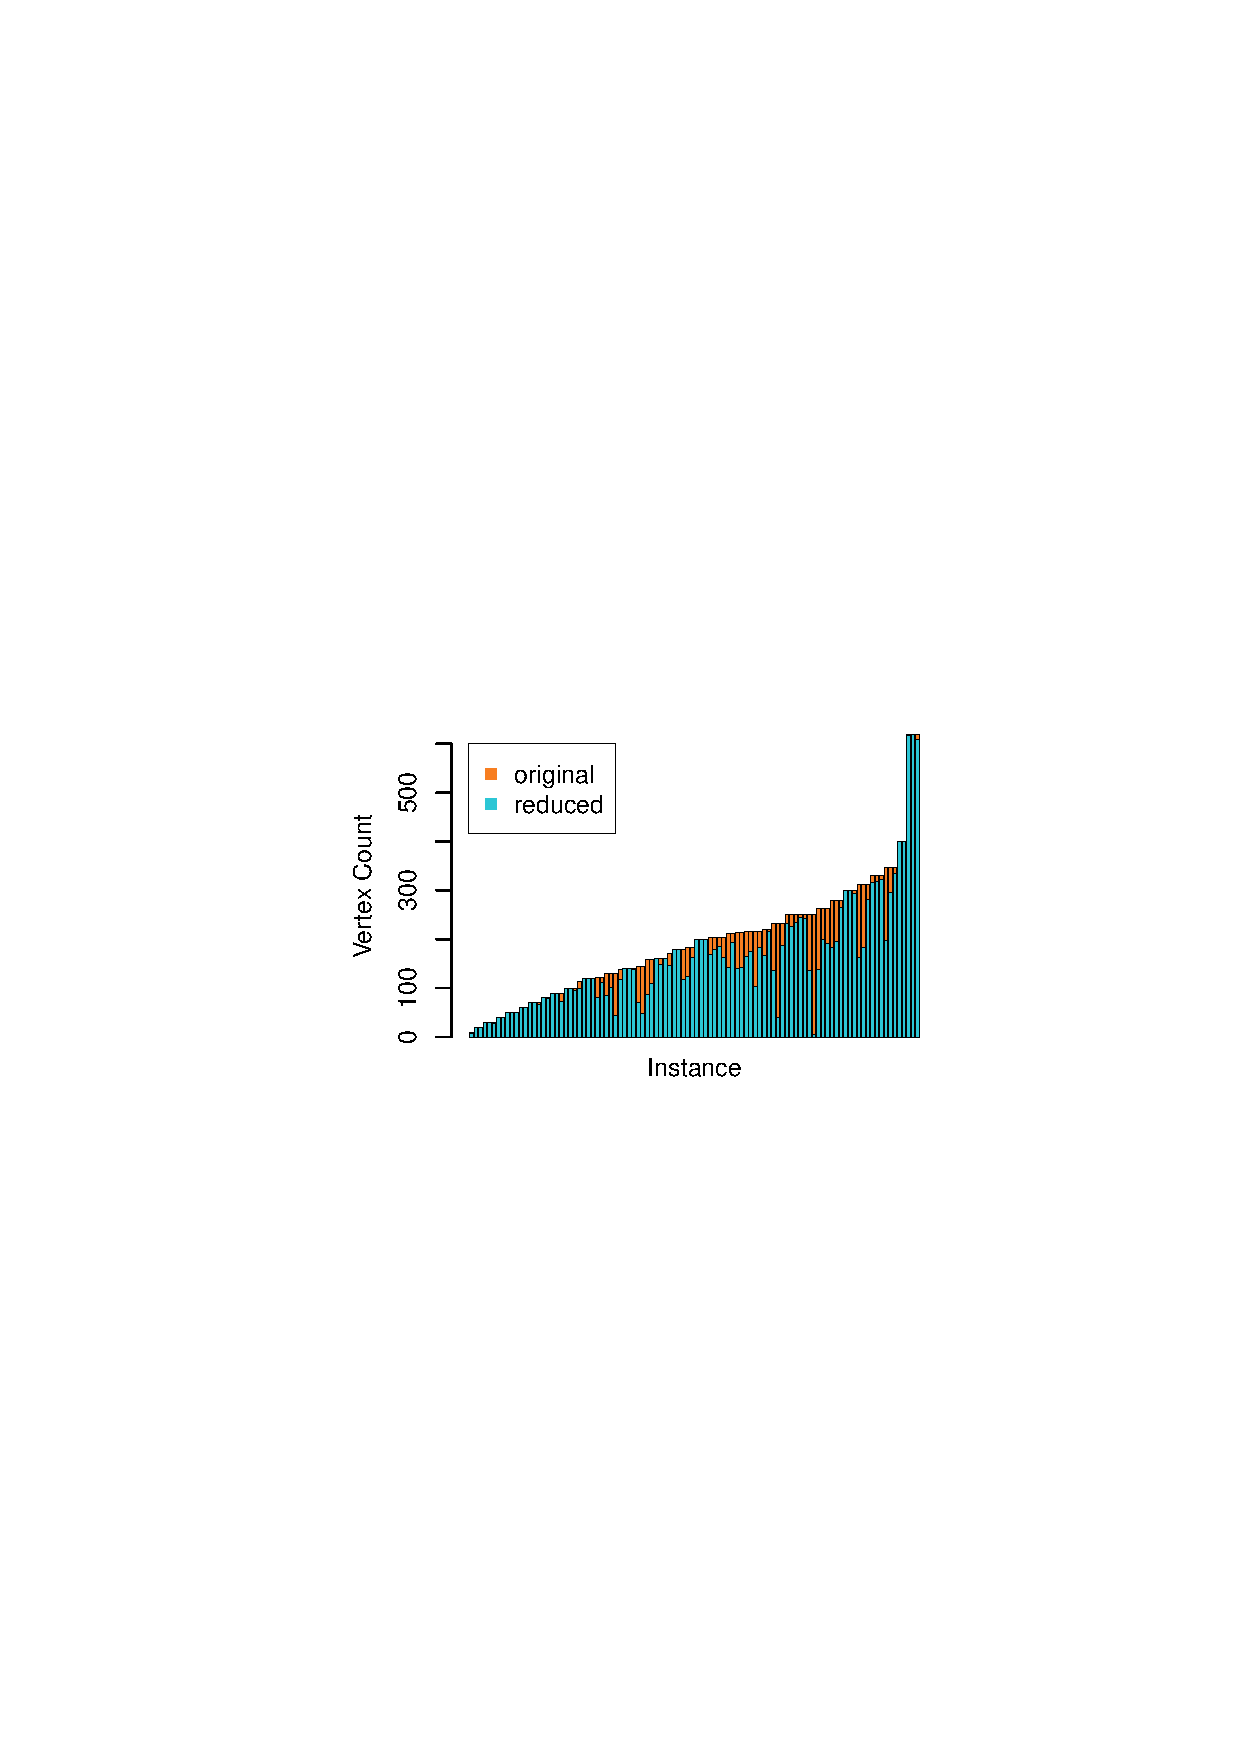
\includegraphics[width=1.0\linewidth]{crit_cliques_absolute}
	\end{subfigure}
	\begin{subfigure}{0.49\textwidth}
		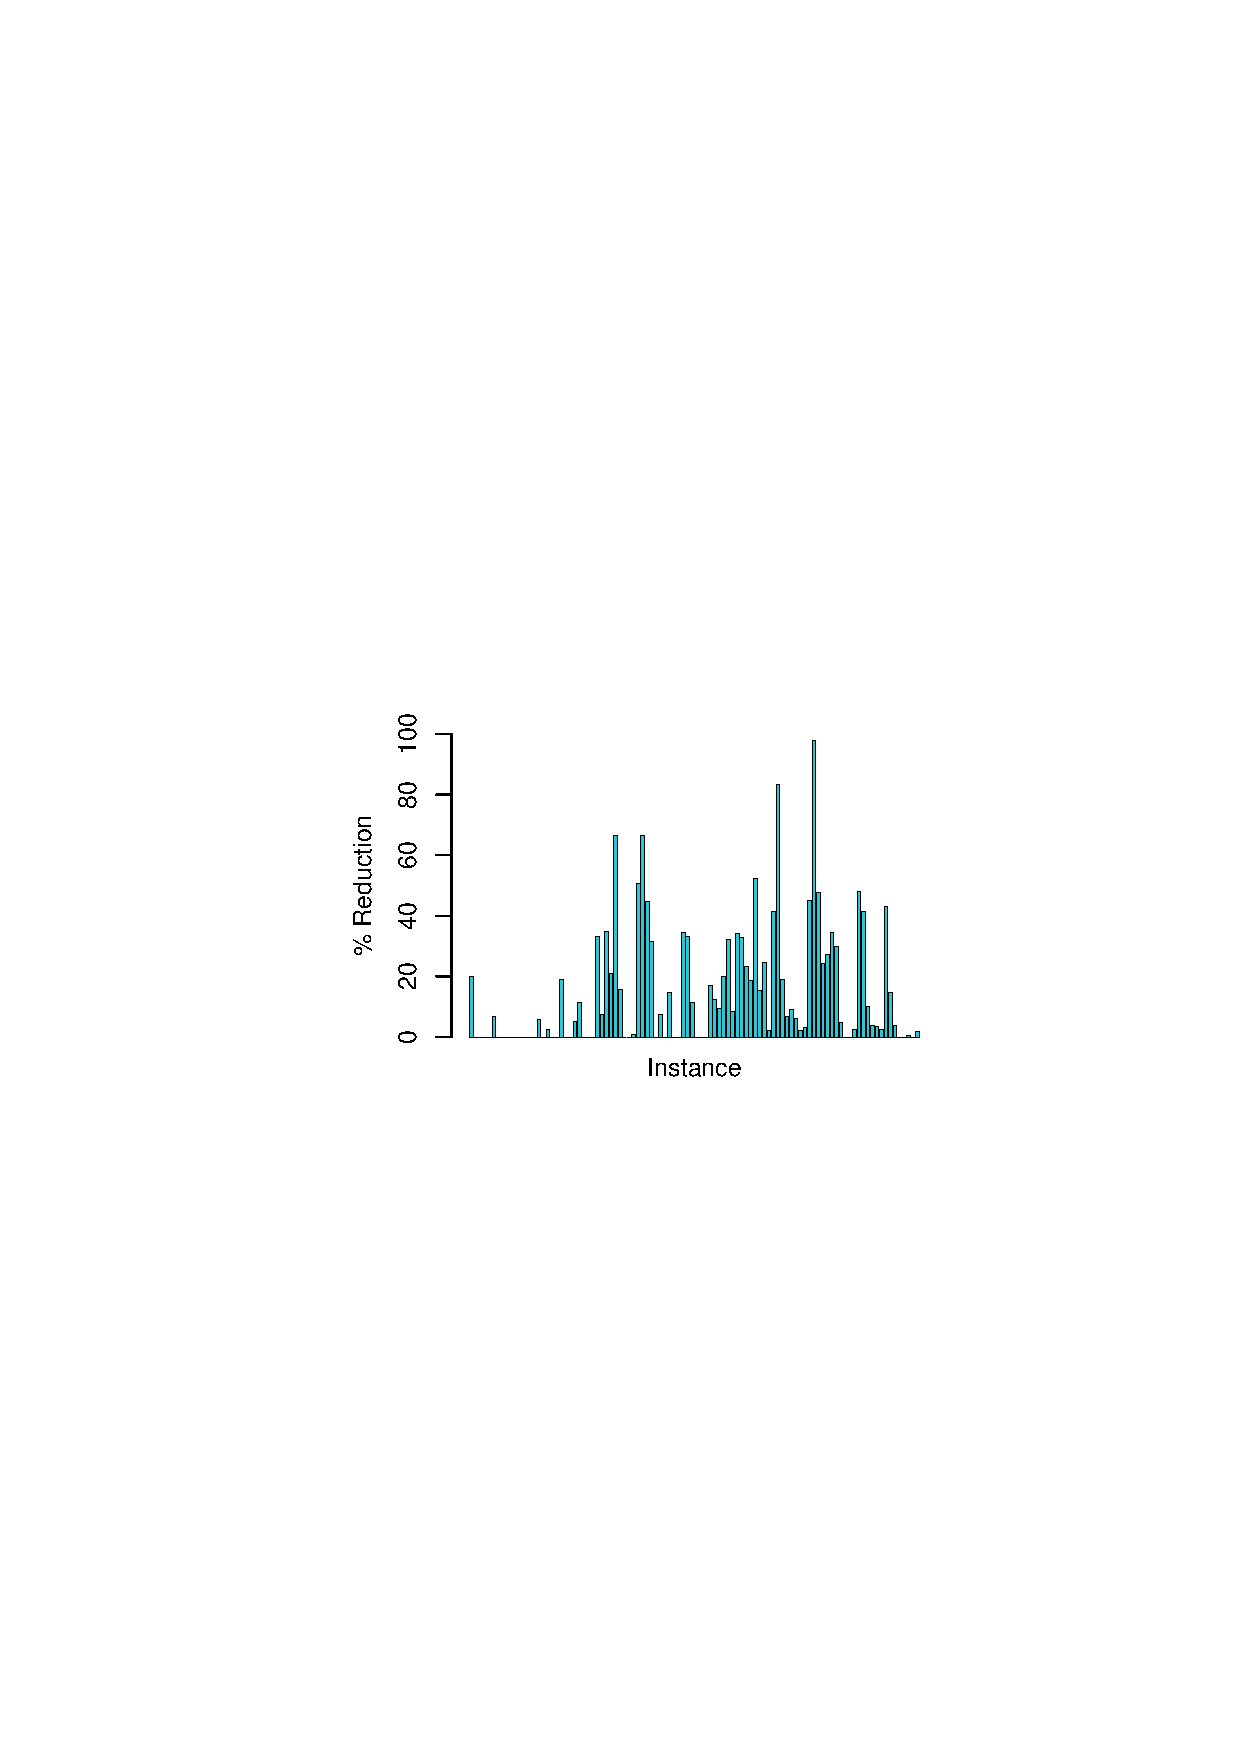
\includegraphics[width=1.0\linewidth]{crit_cliques_percent}
	\end{subfigure}
	\caption{Critical Clique Reduction Effectiveness}
	\label{fig:crit_clique eff}
\end{figure}

We present the same statistics for rules 1--5 applied together and for the complete initial
reduction in figures~\ref{fig:rules1-5 eff} and~\ref{fig:initial eff}. Note that rule 1 forbids
edges instead of merging vertices, so it does not have a direct effect on these graphs (it may still
enable other reduction steps however). We observe that many of the larger peaks occur for the same
instance for both the critical clique reduction and rules 1--5. With figure~\ref{fig:initial eff} we
can see that overall reduction is in fact most effective with all reductions enabled, as expected.
Considering the negligible runtime of the reductions on graphs of the size used in the challenge, it
is definitely reasonable to always run the full set.

\begin{figure}[h]
	\begin{subfigure}{0.49\textwidth}
		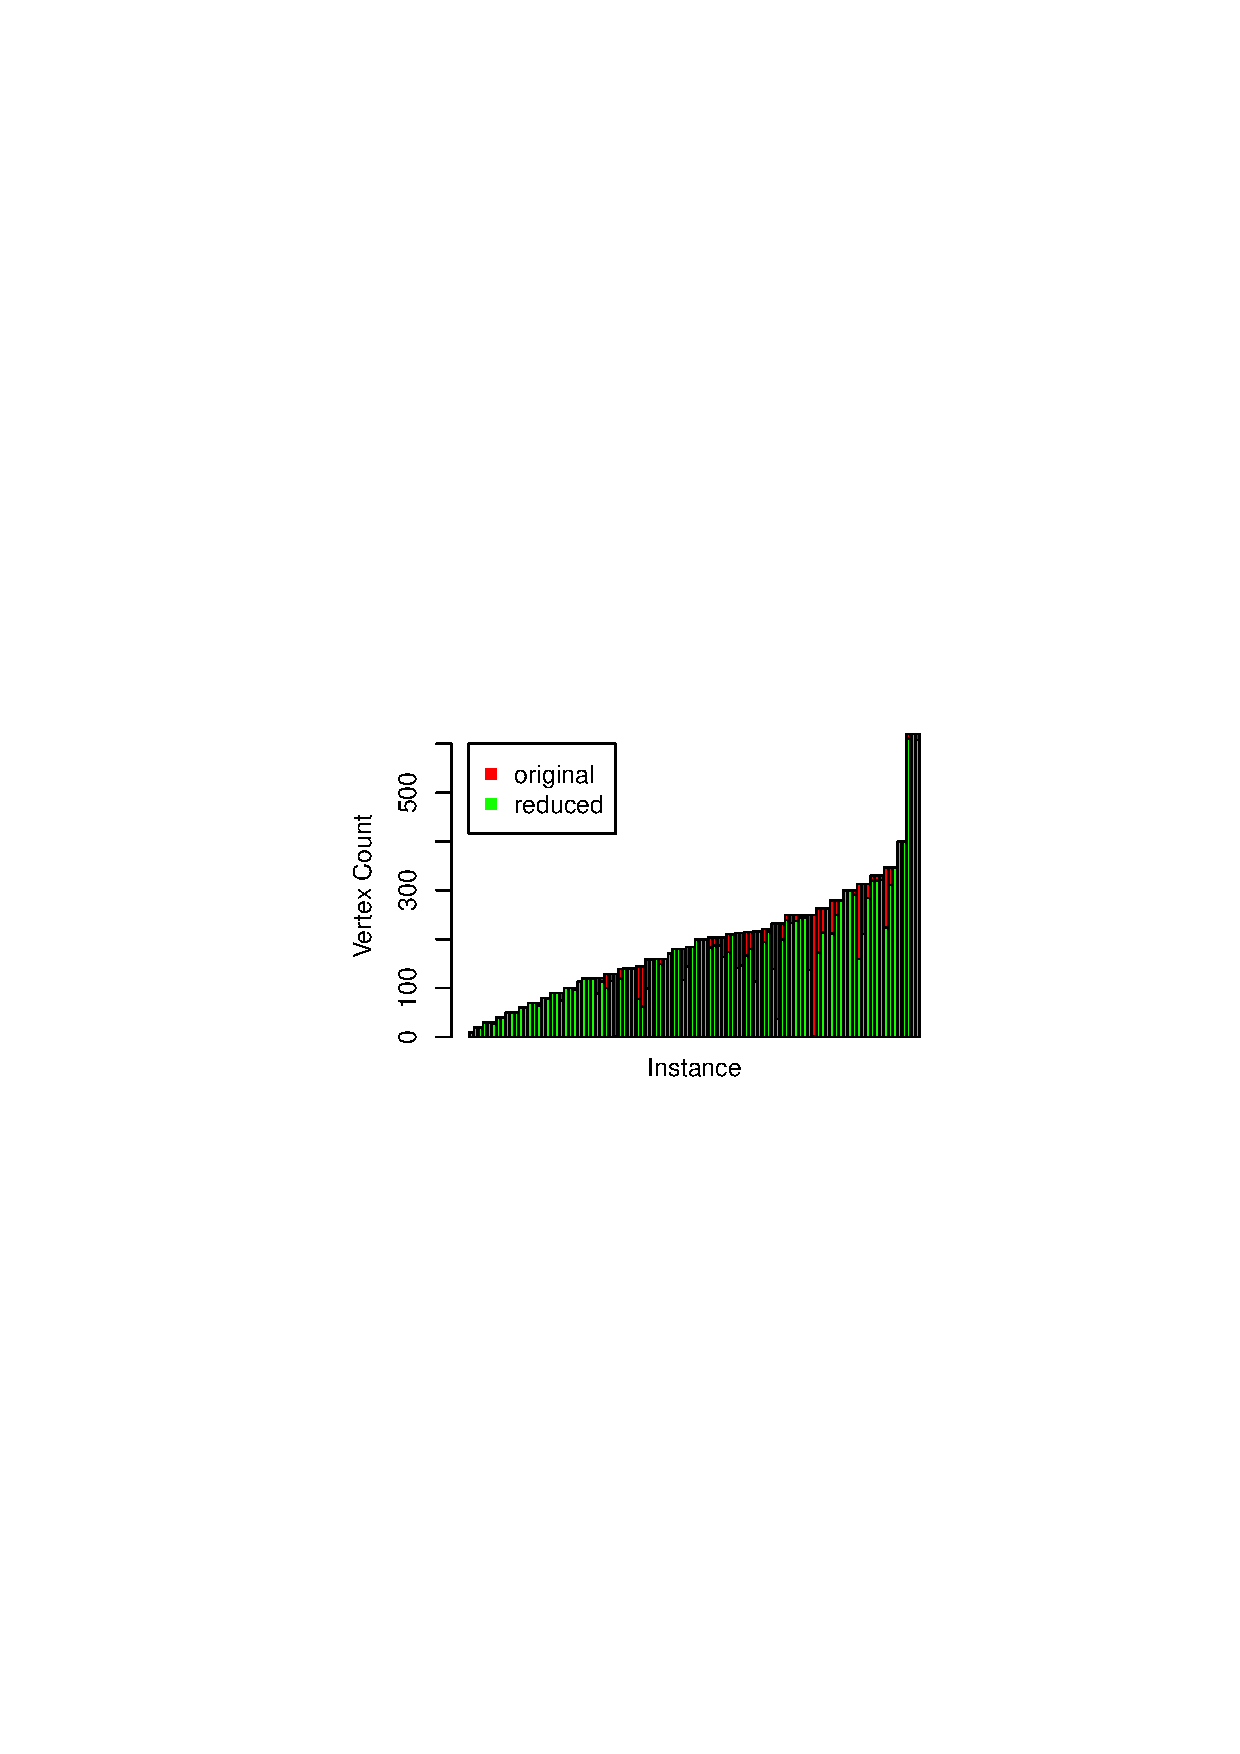
\includegraphics[width=1.0\linewidth]{rules1-5_absolute}
	\end{subfigure}
	\begin{subfigure}{0.49\textwidth}
		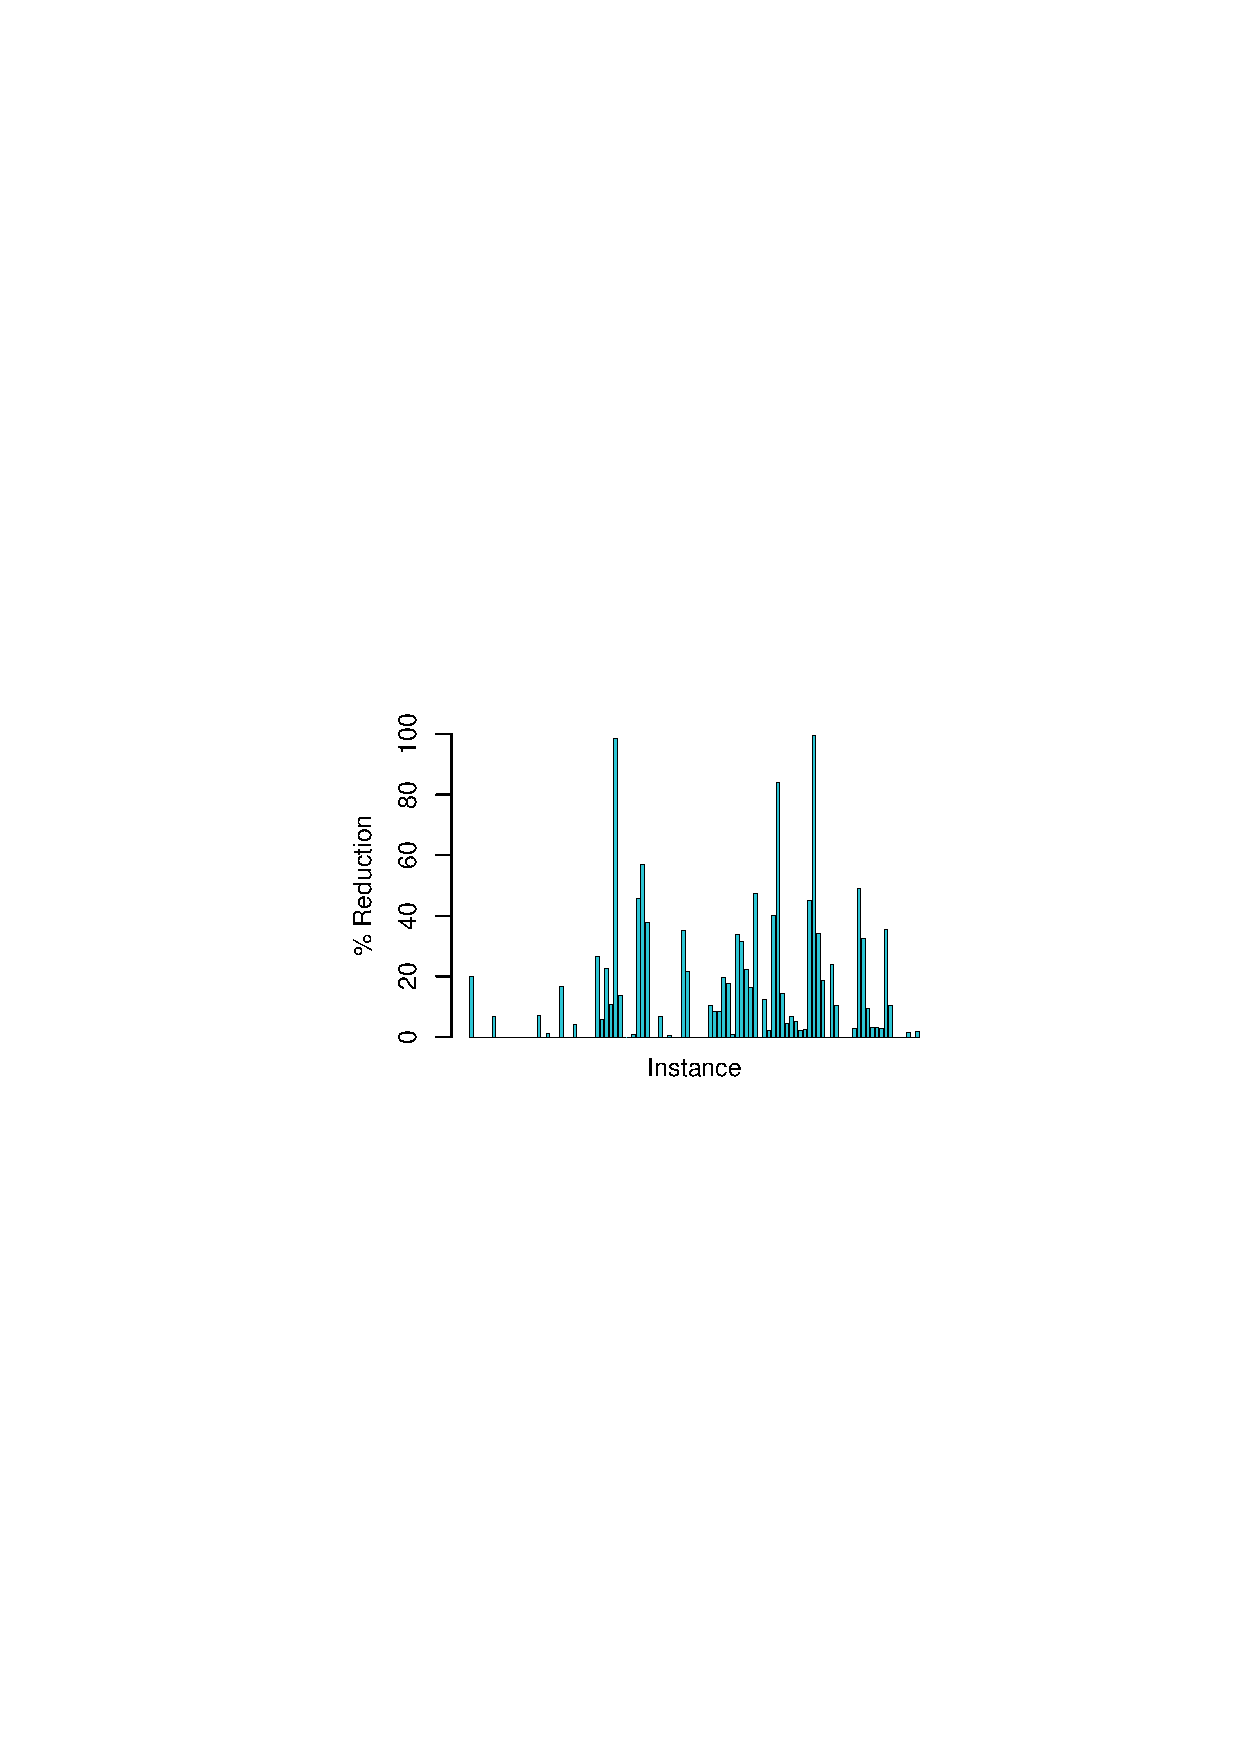
\includegraphics[width=1.0\linewidth]{rules1-5_percent}
	\end{subfigure}
	\caption{Rules 1--5 Effectiveness}
	\label{fig:rules1-5 eff}
\end{figure}

\begin{figure}[h]
	\begin{subfigure}{0.49\textwidth}
		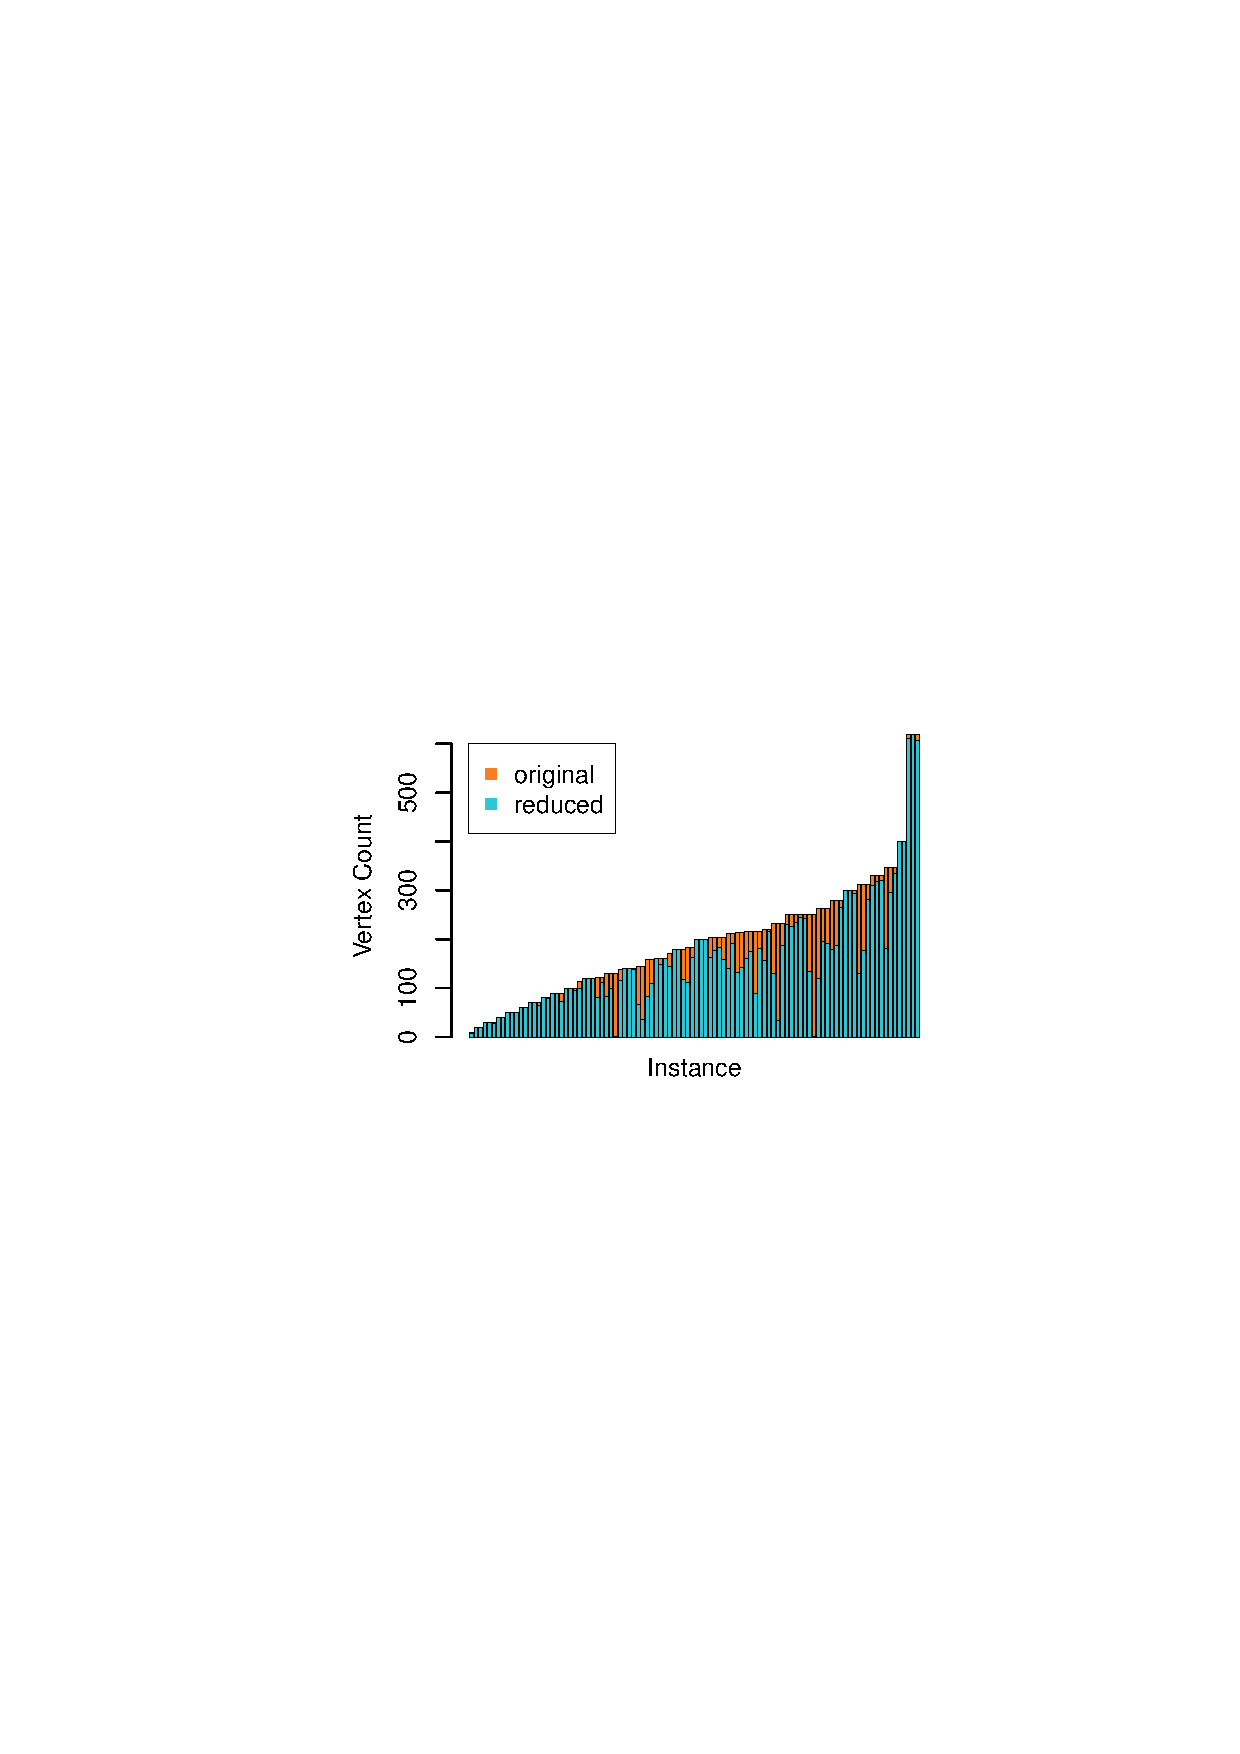
\includegraphics[width=1.0\linewidth]{full_initial_absolute}
	\end{subfigure}
	\begin{subfigure}{0.49\textwidth}
		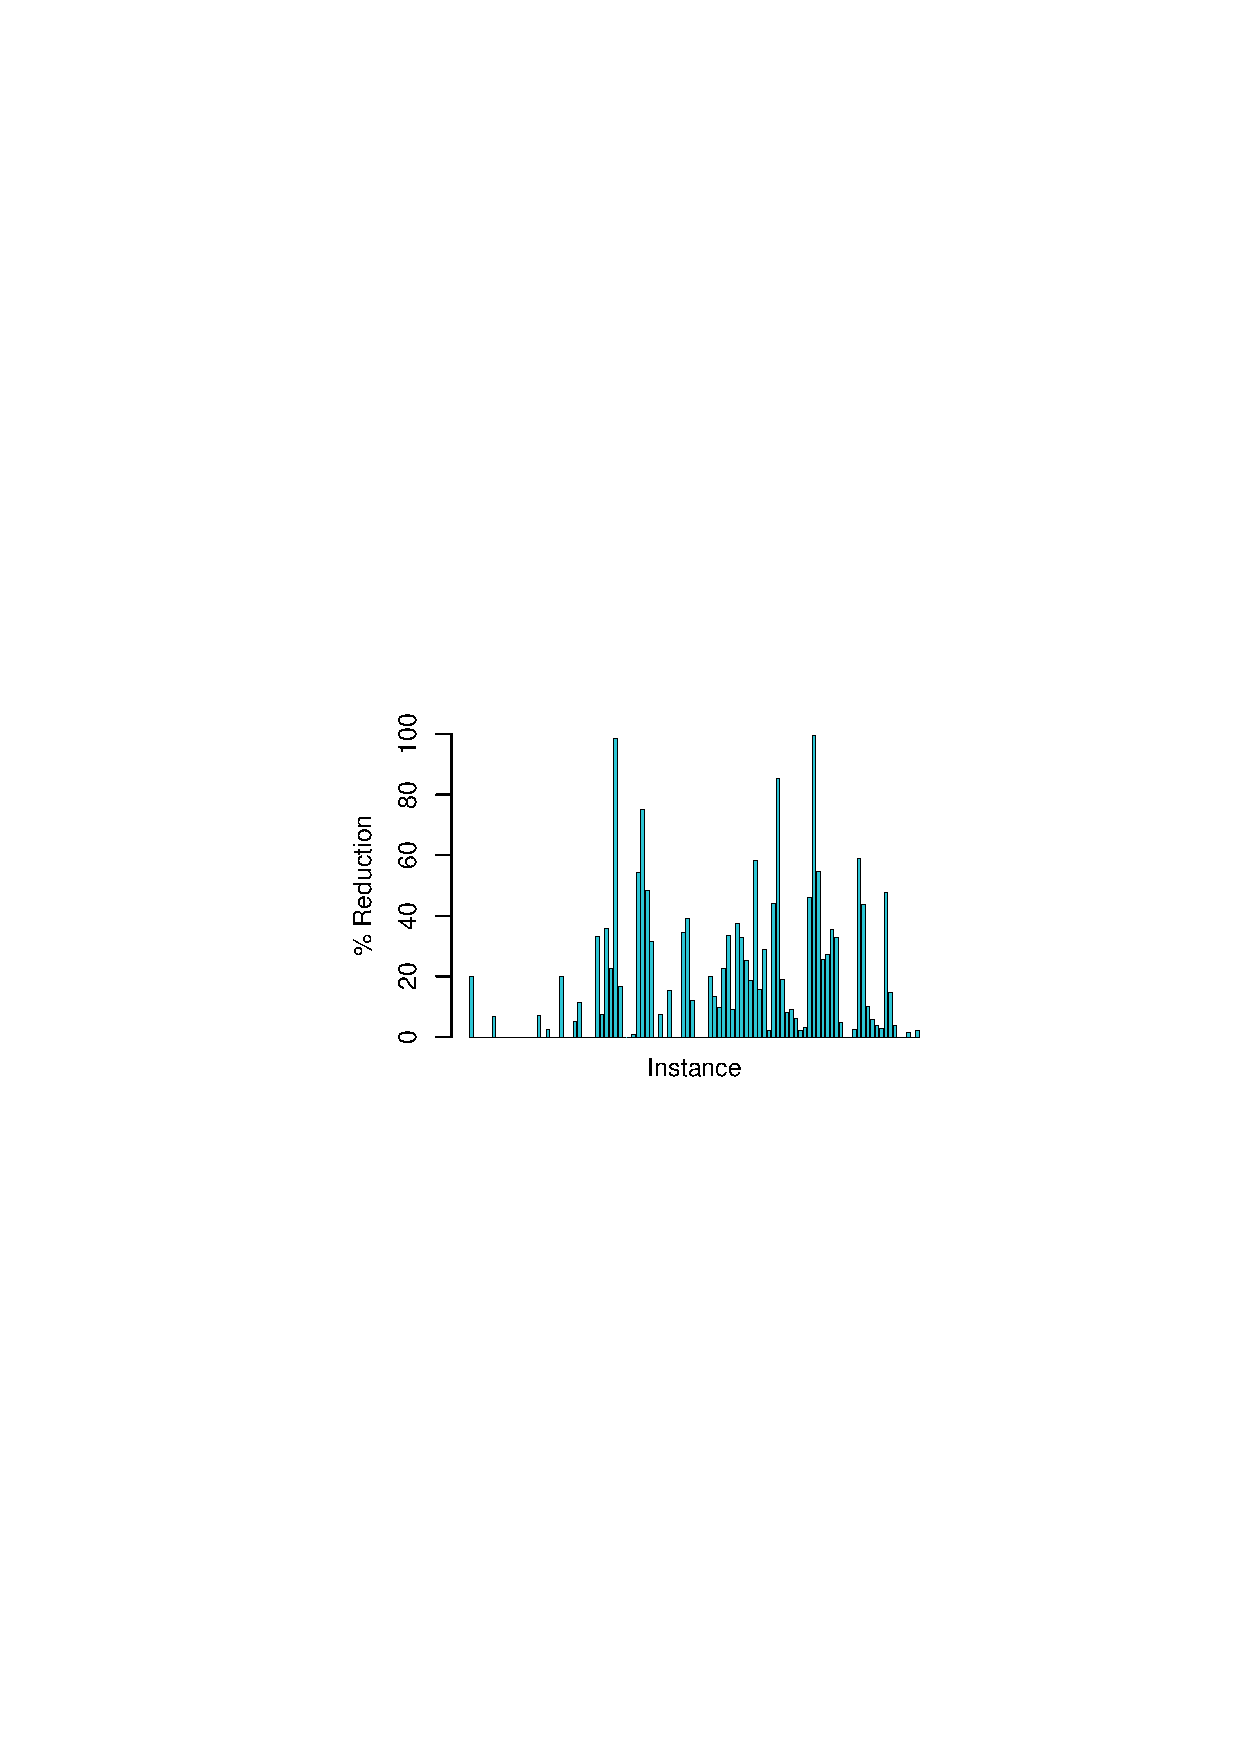
\includegraphics[width=1.0\linewidth]{full_initial_percent}
	\end{subfigure}
	\caption{Full Initial Reduction Effectiveness}
	\label{fig:initial eff}
\end{figure}

An additional factor to consider is that while the effectiveness of the critical clique reduction is
fully captured in the size of the reduced graphs, the same is not true for the other reductions.
While most of them (with the exception of rule 1) also perform merging of vertices as their only
operation on the graph, this can also result in various additional edits, hopefully making the
complete solution easier to find. For an impression of how effective the reductions are in this
regard, in figure~\ref{fig:edits from reduction} we show what percentage of the amount of edits in
an optimal solution is found by the reductions (for the 34 instances we have solved so far).
Comparing the full set of reductions with only using rules 1--5, we can see that while the critical
clique reduction does not produce any edits on its own, the simplified graph it produces is easier
to reduce by the other rules.

\begin{figure}[h]
	\begin{subfigure}{0.49\textwidth}
		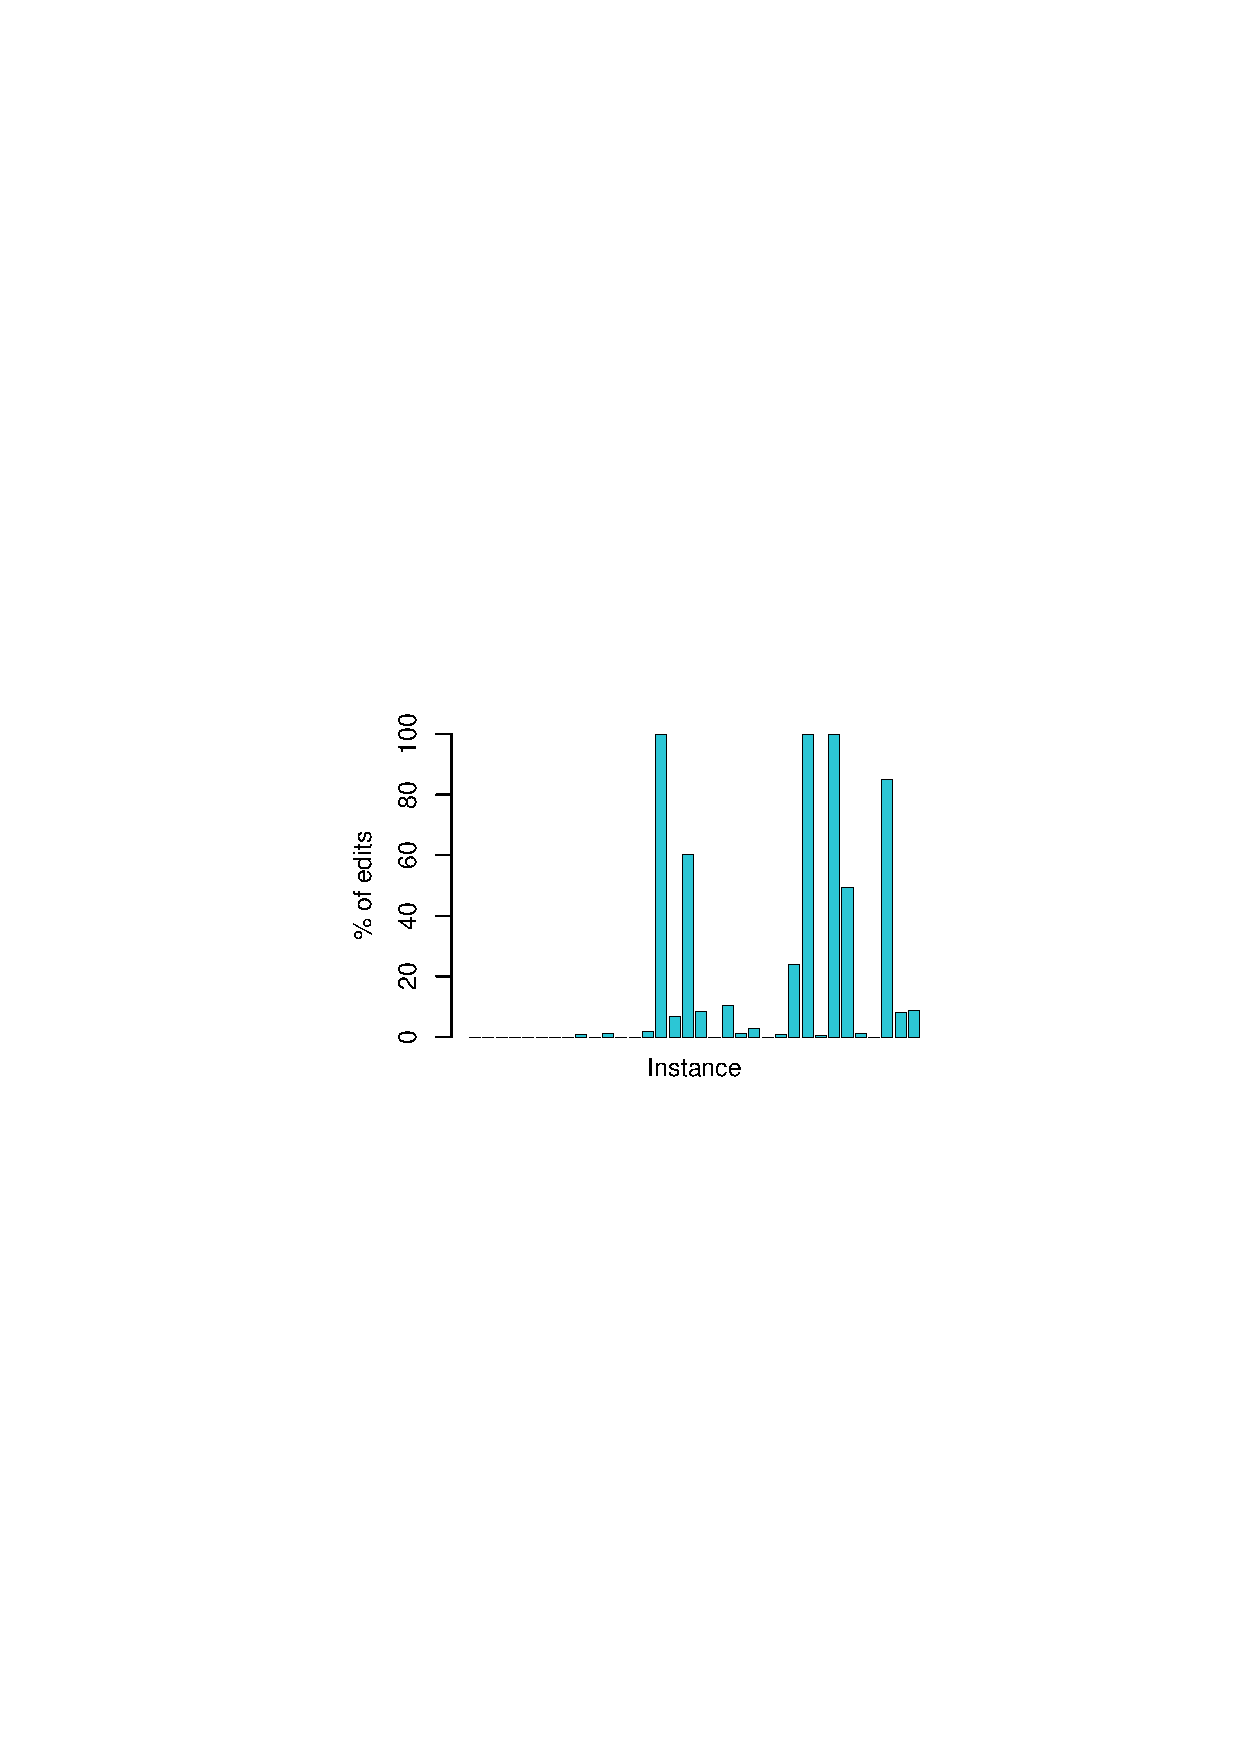
\includegraphics[width=1.0\linewidth]{percent_edits_full}
		\subcaption{Full Initial Reduction}
	\end{subfigure}
	\begin{subfigure}{0.49\textwidth}
		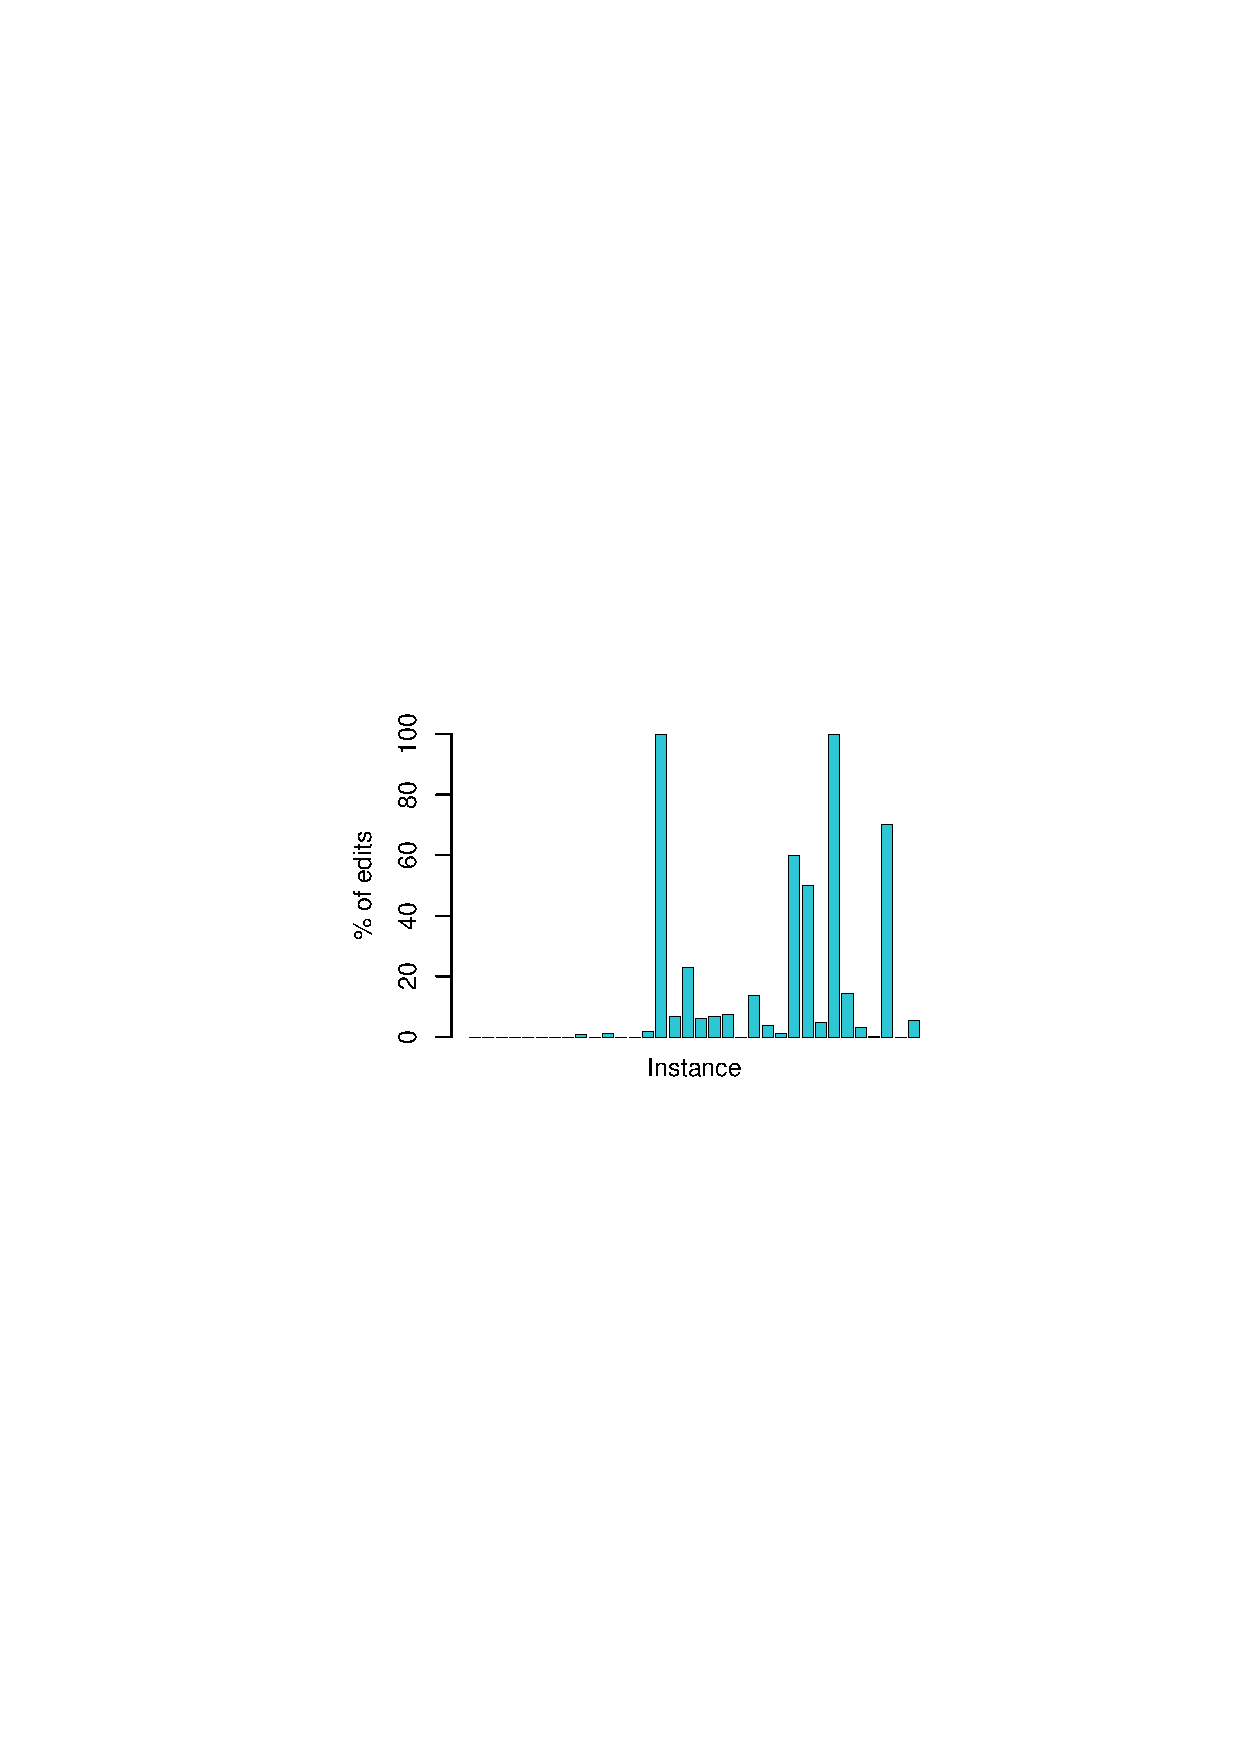
\includegraphics[width=1.0\linewidth]{percent_edits_rules1-5}
		\subcaption{Only rules 1--5}
	\end{subfigure}
	\caption{\% of edits of an optimal solution found by initial reduction steps}
	\label{fig:edits from reduction}
\end{figure}

It is more difficult to precisely measure the effectiveness of reduction steps that happen while
executing the search algorithm. 

% Measurements for interleaved reduction?
% - In the path that led to the solution, how much reduction did the rules do?
%   -> this tells us nothing about how much calculation we were able to skip because of them
% - how much reduction effect they have overall in an execution
%   -> measured in reduction in k? In number of edits made?
%   - to be useful this would probably also require measuring the *total* number of whatever is
%     measured, to compare
% - comparison in runtime with rules disabled or settings tweaked

\todo

\begin{itemize}
	\item Critical clique reduction effectiveness
	\item Initial param-independent reduction effectiveness
	\item Reduction during the search... this is harder/more expensive to measure
	\item Parameter-tuning (reduction intervals)
	\item What techniques provided what kind of benefit as they were introduced, what did we try
		that wasn't worth it?
\end{itemize}

\section{Outlook / Future Possibilities / ?}

\begin{itemize}
	\item multi-threading?
	\item more reductions?
	\item improved initial reduction by making use of upper bounds?
	%\item better branching?
\end{itemize}

\todo Clean the references up a bit, and double-check years etc. Right now these are just whatever
Zotero produced on its own, which is useful to get started quickly. (Clean up formatting too)

\begin{thebibliography}{99}

\bibitem{BenDor}
A. Ben-Dor, R. Shamir, and Z. Yakhini, “Clustering Gene Expression Patterns,” Journal of
Computational Biology, vol. 6, no. 3–4, pp. 281–297, Oct. 1999, doi: 10.1089/106652799318274.

\bibitem{ShamirOverview}
R. Shamir and R. Sharan, “Algorithmic Approaches to Clustering Gene Expression Data,” in Current
Topics in Computational Biology, 2001, pp. 269–300.

\bibitem{ShamirModifications}
R. Shamir, R. Sharan, and D. Tsur, “Cluster graph modification problems,” Discrete Applied
Mathematics, vol. 144, no. 1, pp. 173–182, Nov. 2004, doi: 10.1016/j.dam.2004.01.007.

\bibitem{Krivanek}
M. Křivánek and J. Morávek, “NP-hard problems in hierarchical-tree clustering,” Acta Informatica,
vol. 23, no. 3, pp. 311–323, Jun. 1986, doi: 10.1007/BF00289116.

\bibitem{Gramm}
J. Gramm, J. Guo, F. Hüffner, and R. Niedermeier, “Graph-Modeled Data Clustering: Fixed-Parameter
Algorithms for Clique Generation,” in Algorithms and Complexity, vol. 2653, R. Petreschi, G.
Persiano, and R. Silvestri, Eds. Berlin, Heidelberg: Springer Berlin Heidelberg, 2003, pp. 108–119.

\bibitem{Bansal}
N. Bansal, A. Blum, and S. Chawla, “Correlation Clustering,” Machine Learning, vol. 56, no. 1,
pp. 89–113, Jul. 2004, doi: 10.1023/B:MACH.0000033116.57574.95.

\bibitem{Charikar}
M. Charikar, V. Guruswami, and A. Wirth, “Clustering with qualitative information,” Journal of
Computer and System Sciences, vol. 71, no. 3, pp. 360–383, Oct. 2005, doi:
10.1016/j.jcss.2004.10.012.

\bibitem{Cai}
L. Cai, “Fixed-parameter tractability of graph modification problems for hereditary properties,”
Information Processing Letters, vol. 58, no. 4, pp. 171–176, May 1996, doi:
10.1016/0020-0190(96)00050-6.

\bibitem{Dehne}
F. Dehne, M. A. Langston, X. Luo, S. Pitre, P. Shaw, and Y. Zhang, “The Cluster Editing Problem:
Implementations and Experiments,” in Parameterized and Exact Computation, Berlin, Heidelberg, 2006,
pp. 13–24, doi: 10.1007/11847250\_2.

\bibitem{Rahmann}
S. Rahmann, T. Wittkop, J. Baumbach, M. Martin, A. Truß, and S. Böcker, “Exact and Heuristic
Algorithms for Weighted Cluster Editing,” in Computational Systems Bioinformatics, University of
California, San Diego, USA, Sep. 2007, pp. 391–401, doi: 10.1142/9781860948732\_0040.

\bibitem{AnApproach}
S. Böcker, S. Briesemeister, Q. A. Bui, and A. Truß, “A Fixed-Parameter Approach for Weighted
Cluster Editing,” 2008, doi: 10.1142/9781848161092\_0023.

\bibitem{GoingWeighted}
S. Böcker, S. Briesemeister, Q. B. A. Bui, and A. Truss, “Going Weighted: Parameterized
Algorithms for Cluster Editing,” in Combinatorial Optimization and Applications, Berlin, Heidelberg,
2008, pp. 1–12, doi: 10.1007/978-3-540-85097-7\_1.

% TODO: We mention this as being from 2008 in the text, should cite the actual version published
% then probably.
\bibitem{ExactAlgos}
S. Böcker, S. Briesemeister, and G. W. Klau, “Exact Algorithms for Cluster Editing: Evaluation
and Experiments,” Algorithmica, vol. 60, no. 2, pp. 316–334, Jun. 2011, doi:
10.1007/s00453-009-9339-7.

\bibitem{EvenFaster}
S. Böcker and P. Damaschke, “Even faster parameterized cluster deletion and cluster editing,”
Information Processing Letters, vol. 111, no. 14, pp. 717–721, Jul. 2011, doi:
10.1016/j.ipl.2011.05.003.

\bibitem{GoldenRatio}
S. Böcker, “A golden ratio parameterized algorithm for Cluster Editing,” Journal of Discrete
Algorithms, vol. 16, pp. 79–89, Oct. 2012, doi: 10.1016/j.jda.2012.04.005.

\bibitem{BoundedDegree}
P. Damaschke, “Bounded-Degree Techniques Accelerate Some Parameterized Graph Algorithms,” in
Parameterized and Exact Computation, vol. 5917, J. Chen and F. V. Fomin, Eds. Berlin, Heidelberg:
Springer Berlin Heidelberg, 2009, pp. 98–109.

\bibitem{Protti}
F. Protti, M. D. da Silva, and J. L. Szwarcfiter, “Applying Modular Decomposition to
Parameterized Bicluster Editing,” in Parameterized and Exact Computation, Sep. 2006, pp. 1–12, doi:
10.1007/11847250\_1.

\bibitem{Fellows}
M. Fellows, M. Langston, F. Rosamond, and P. Shaw, “Efficient Parameterized Preprocessing for
Cluster Editing,” in Fundamentals of Computation Theory, vol. 4639, E. Csuhaj-Varjú and Z. Ésik,
Eds. Berlin, Heidelberg: Springer Berlin Heidelberg, 2007, pp. 312–321.

\bibitem{Guo}
J. Guo, “A more effective linear kernelization for cluster editing,” Theoretical
Computer Science, vol. 410, no. 8, pp. 718–726, Mar. 2009, doi: 10.1016/j.tcs.2008.10.021.

\bibitem{ChenMeng}
J. Chen and J. Meng, “A 2k kernel for the cluster editing problem,” Journal of Computer and
System Sciences, vol. 78, no. 1, pp. 211–220, Jan. 2012, doi: 10.1016/j.jcss.2011.04.001.

\bibitem{Rust}
“Rust Programming Language.” https://www.rust-lang.org/ (accessed Apr. 20, 2021).

\bibitem{AbuKhzam}
F. N. Abu-Khzam, K. A. Jahed, and A. E. Mouawad, “A Hybrid Graph Representation for Exact Graph
Algorithms,” arXiv:1404.6399 [cs], Apr. 2014, Accessed: Apr. 20, 2021. [Online]. Available:
http://arxiv.org/abs/1404.6399.

\end{thebibliography}

\end{document}
